\documentclass[journal]{IEEEtran}
\usepackage{cite}
\usepackage{amsmath,amssymb}
\usepackage{graphicx}
\usepackage{booktabs}
\usepackage{textcomp}
\usepackage{url}
% keep command names and the ISA name from breaking across lines
\newcommand{\cmd}[1]{\mbox{\texttt{#1}}}
\hyphenation{RISC-V}
\renewcommand{\topfraction}{0.92}
\renewcommand{\bottomfraction}{0.85}
\renewcommand{\textfraction}{0.06}
\renewcommand{\floatpagefraction}{0.75}

\begin{document}

\title{Verifying the RISC-V IOMMU: An Open Verification Environment\\and a Fault-Injection Evaluation}
\author{Maulik~Timbadiya,~\IEEEmembership{Independent Researcher}}
\markboth{Verifying the RISC-V IOMMU}{Timbadiya}
\maketitle

\begin{abstract}
The RISC-V IOMMU specification reached version 1.0 in 2024 and the first
open-source RTL implementations have appeared. Verification work on them has
begun, but no environment for one has been published that a reader can obtain
and run, and the leading open implementation ships with no testbench in its
repository. We report an open, licence-free verification
environment for that IP and an evaluation of what it actually catches. The
environment drives all four AXI interfaces of the device, serves its
implicit page-table, command and fault-queue accesses from a memory model,
and checks every translation against an independent software walker; it is
1{,}144 lines of SystemVerilog, builds in 2.4~s and runs 56 checks in 5~ms
using Verilator alone. We evaluate it by injecting eleven semantically
meaningful IOMMU faults into the RTL. Against that fixed fault set, the core
functional suite detects six of eleven;
the survivors identified concrete blind spots --- page-table permission bits,
reserved-bit encodings and second-stage translation --- and the tests written
to close them bring detection to eleven of eleven. We report two findings
about the IP: it cannot be linted as published because a dependency is absent,
and, with the fault queue disabled, eight faulting device accesses leave the
IOMMU unresponsive and a previously valid translation fails. We also report a
methodology result we think is more broadly useful: during development a
protocol-violating bus driver produced three plausible, reproducible and
entirely false IP defects, which argues for protocol checking on the stimulus
side of a testbench and not only on the device under test.
\end{abstract}

\begin{IEEEkeywords}
IOMMU, RISC-V, functional verification, fault injection, mutation testing,
address translation, SystemVerilog, open-source hardware.
\end{IEEEkeywords}

\section{Introduction}

\IEEEPARstart{A}{n} IOMMU stands between devices and memory. It translates the
addresses a device emits, enforces the permissions of the domain that owns the
device, and is the mechanism by which an operating system or hypervisor confines
a DMA-capable peripheral. Because it is a confinement mechanism, a defect in it
is a containment failure: a device may reach memory it was never granted, or a
stale cached translation may outlive the mapping it came from.

The RISC-V IOMMU specification reached version~1.0, and open RTL
implementations have followed. The most complete of these is the IP published by
Zero-Day Labs~\cite{rviommu}, which implements device-directory walks, two-stage
Sv39/Sv39x4 translation, an IOTLB and directory caches, a command queue and a
fault queue. Its own documentation states that the IP ``is not formally
verified'' and is ``very likely to have bugs.'' It ships no testbench: its
makefile invokes Verilator in \texttt{--lint-only} mode.

That gap is the subject of this article, and it needs stating precisely,
because it is not that nobody has verified an IOMMU. Zero-Day Labs and
10xEngineers reported a collaborative verification effort on this very IP at the
RISC-V Summit in 2024, citing 85\,\% of coverage targets met and several RTL
defects found~\cite{zdl10x}; and standalone IOMMU verification with a reference
model has been published before, for the Elbrus-6 processor~\cite{elbrus}. What
is missing is different and more mundane: an environment a reader can obtain,
build and run. The 10xEngineers work is, as far as we can determine, not
publicly available, and the Elbrus work targets a proprietary device. There is
also a substantial literature on verifying RISC-V \emph{cores}---random
instruction generators, reference-model co-simulation, coverage
closure~\cite{riscvdv,corevverif}---and a separate literature on verifying
address-translation \emph{ordering} for CPU MMUs~\cite{coatcheck,transform}.
This article does not propose a new verification theory. It reports what it takes to build a usable environment for this class of
device, and---more importantly---measures how much of the device's behaviour
that environment actually exercises, using fault injection rather than assertion
counts or line coverage.

\subsection{Contributions}
\begin{enumerate}
\item An open verification environment for the RISC-V IOMMU that needs only
      Verilator, Yosys is not required, and no commercial licence. It drives the
      programming, device-request, completion and data-structure interfaces, and
      checks translations against an independent walker.
\item A fault-injection evaluation with eleven injected IOMMU defects, and the
      ablation that matters: against a fixed set of eleven faults, the core
      suite catches six, and the tests written to close those gaps catch all
      eleven.
\item Two reproducible findings about the IP: it cannot be linted as published,
      and disabling the fault queue lets a faulting device render the IOMMU
      unresponsive.
\item A methodology result: a bus driver that violated the AXI handshake
      manufactured three convincing false defects in the device under test.
\end{enumerate}

\section{Background}

\subsection{What the device does}
A device issues a transaction carrying a \emph{device identifier}. The IOMMU
uses that identifier to walk a device-directory table (DDT) in memory and
obtain a device context, which names the translation structures for that device:
a first-stage table (Sv39, the device's own virtual addresses), a second-stage
table (Sv39x4, the guest-to-supervisor mapping) or neither, in which case the
transaction passes through. The resulting translation is cached in an IOTLB, and
the device context itself in a directory cache.

Because those caches are filled from memory the host also writes, software must
be able to invalidate them. The IOMMU exposes a command queue; software enqueues
\cmd{IOTINVAL.VMA} to invalidate translations and \cmd{IOFENCE.C} to learn
when previous commands have taken effect. Faults---an invalid device context, a
missing page-table entry, a permission violation---are reported by appending a
record to a fault queue and by aborting the offending transaction.

\subsection{Why this is awkward to verify}
Three properties make an IOMMU harder to drive than a core. First, its stimulus
is not instructions but bus transactions on one port, with the response
appearing on a \emph{different} port: the translated transaction is issued by the
IOMMU as a master, so the quantity under test---the translated address---is
observed on an interface the testbench must implement as a slave. Second, most
of its behaviour depends on data structures in memory, so a testbench must
construct valid device-directory and page-table images before any stimulus is
meaningful. Third, its caches make behaviour history-dependent: the same
transaction is correct or incorrect depending on what was invalidated before it.

\section{Related Work}
Verification of RISC-V cores is well served. \texttt{riscv-dv}~\cite{riscvdv}
generates constrained-random instruction streams and \texttt{core-v-verif}
provides UVM environments with reference-model co-simulation~\cite{corevverif};
both target cores, require a commercial simulator for their UVM components, and
do not address an IOMMU.

IOMMU verification has been attempted before, and we want to be accurate about
what is new here rather than claim a vacant field. Petrykin \emph{et
al.}~\cite{elbrus} built a standalone test system and reference model for the
IOMMU of the Elbrus-6 processor, covering dynamically generated translation
tables and two-level translation---close in intent to what we report, on a
proprietary device, with no artifact available. Closer still, Zero-Day Labs and
10xEngineers presented a collaborative verification effort on the very IP we
target at the RISC-V Summit in 2024~\cite{zdl10x}, reporting 85\,\% of coverage
targets met and several RTL defects and design issues found. We could not locate
a public repository for that environment.

Our contribution is therefore narrower than ``the first verification of a RISC-V
IOMMU,'' and we do not claim that. It is an environment that is open, builds
with free tools, runs in seconds, and reproduces every number in this article
from a single command---together with a measurement, by fault injection, of what
it would and would not have caught. Where the 10xEngineers effort reports
coverage, we deliberately report detection instead, for the reason set out in
Section~VII.

Address translation has been studied from the ordering side. COATCheck models
memory ordering at the hardware--OS interface including translation
events~\cite{coatcheck}, and TransForm synthesises litmus tests for such
``transistency'' models~\cite{transform}. RTLCheck verifies that RTL satisfies
the microarchitectural axioms a consistency proof
assumes~\cite{rtlcheck}. These concern a CPU's MMU and its interaction with
software; none targets a device-side IOMMU, and none constructs a functional
verification environment for one. The invalidation-ordering subset of that gap
is the subject of a companion article~\cite{companionB}; here we are concerned
with the environment and with what fault injection says about the suite as a
whole.

Fault injection as a way of measuring a test suite is long established in
software as mutation testing, and has been applied to hardware description
languages to assess verification quality. We use it here not to claim novelty in
the technique but because it answers the question that matters for a new
environment: not how many lines were executed, but which defects would survive.

\section{Device Under Test}
We target the Zero-Day Labs RISC-V IOMMU IP~\cite{rviommu} at commit
\texttt{18ad30a}: 75 SystemVerilog files, 25{,}778 lines, Apache-2.0 and
Solderpad licensed. It implements one-, two- and three-level device directories,
Sv39 first-stage and Sv39x4 second-stage translation with superpages, a
fully-associative IOTLB, device- and process-directory caches, the command and
fault queues, wired and message-signalled interrupts, and performance counters.
It does not implement the PCIe ATS command set.

The IP exposes four AXI4 interfaces: a slave port on which devices issue
transactions, a master port on which translated transactions leave, a master
port for its own implicit accesses (directory walks, page-table walks, queue
accesses), and a programming slave port.

\subsection{It cannot be linted as published}
Our first observation is prosaic and immediate. The register map includes
\texttt{common\_cells/assertions.svh}, which the repository does not vendor, so
the IP's own lint flow fails on a clean checkout. Supplying the upstream
lowRISC header does not fix it: that header defines \texttt{ASSERT\_RPT} with
two arguments where this IP's RTL uses one, and the build fails on a macro
arity error. We resolved it by forwarding the missing path to the IP's own
bundled \texttt{assertions.svh}, which keeps one self-consistent set of macros.
With that one file supplied, the IP lints clean and elaborates under Verilator.

\section{The Verification Environment}

\begin{figure*}[!t]
\centering
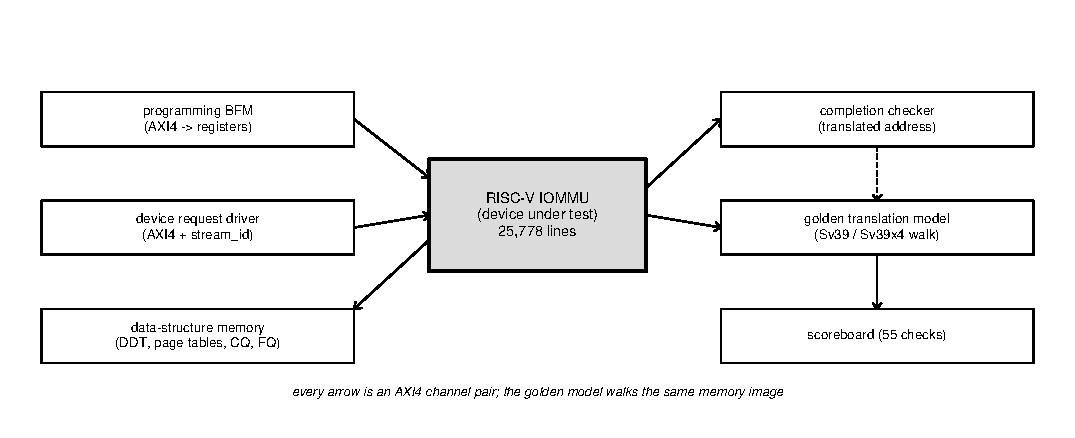
\includegraphics[width=\textwidth]{figures/figA1_env.pdf}
\caption{Environment structure. The translated address---the quantity under
test---is observed on the completion port, which the testbench implements as a
slave, and compared against an independent walk of the same memory image.}
\label{fig:env}
\end{figure*}

Fig.~\ref{fig:env} shows the structure. Four components surround the device.

\emph{A programming driver} performs register reads and writes over AXI4. It
supports both 8-byte and 4-byte accesses, which matters: several IOMMU registers
are 32 bits wide and the \texttt{ddtp} register commits only when both of its
32-bit halves have been written, so an environment that can only issue 8-byte
accesses cannot program the device correctly, and one that masks sub-word
addresses to the 8-byte boundary will write the neighbouring register.

\emph{A data-structure memory model} serves the IOMMU's implicit accesses as an
AXI4 slave over a 512~KiB sparse image. Every structure the device reads---the
device directory, both levels of page tables, the command queue---and every
structure it writes---fault records, fence completion words---lives in this
image, which the testbench also builds and inspects directly.

\emph{A device request driver} issues reads and writes on the translation
request port, carrying a device identifier in the AXI user-defined fields.

\emph{A completion checker} implements the master port as a slave, recording the
translated address of every transaction the IOMMU forwards.

\emph{An independent walker} re-implements the Sv39 walk in the testbench,
reading the same memory image, and yields the address each transaction should
produce. Checks compare the observed translated address against it rather than
against a constant, so a test remains valid when the page tables change.

\subsection{Constructing the data structures}
Nothing in the device is reachable until memory contains structures it accepts,
and the encodings are unforgiving. A base-format device context is four 64-bit
words---translation control, second-stage pointer, translation attributes,
first-stage pointer---placed at \texttt{DDT\_BASE} $+$ device identifier
$\times$ 32 in one-level mode. Only bit~0 of the first word, the valid bit, must
be set for a minimal context; the two pointer words select translation mode in
their top four bits, so leaving both zero yields a valid device whose
transactions pass through untranslated. That configuration is the smallest
end-to-end test in the suite and the one we brought up first: it exercises
register programming, the directory walk and the completion path while removing
page tables from the problem.

First-stage page-table entries follow the Sv39 format: the physical page number
occupies bits 53:10 and the permission bits occupy the low byte. Our builder
writes three levels, with non-leaf entries carrying only the valid bit and the
leaf carrying valid, read, write, user, accessed and dirty. The second stage
uses Sv39x4, whose root table is 16~KiB and is indexed by eleven bits of the
guest address rather than nine; getting that index width wrong produces a walk
that reads a plausible but wrong table entry, which is why the second-stage test
checks the number of implicit accesses as well as the final address.

\subsection{Command queue mechanics}
The command queue is a power-of-two ring of 16-byte entries whose base and size
are programmed together, with software advancing a tail index and the IOMMU
advancing a head index. Two details matter for a testbench. The tail index must
wrap: we initially incremented it without wrapping, which wrote commands past
the end of the queue and left the device with a tail index outside the ring, so
invalidation silently stopped working while every earlier test still passed.
And the queue's registers are 32 bits wide and adjacent, so an 8-byte write
aimed at the tail also writes the head.

\cmd{IOFENCE.C} carries an address and a data word; when the address-valid
bit is set the IOMMU writes that data to that address once preceding commands
have taken effect. Because the address field is expressed in units of four
bytes, the testbench polls its own memory image for the data word and uses its
appearance as the ordering reference point for the invalidation tests.

\subsection{Observing responses correctly}
Both drivers determine completion by counting channel handshakes rather than by
sampling a \texttt{valid} level. This is not fastidiousness. An early version
sampled levels, and after a faulting transaction it mistook a stale response for
its own, producing tests that reported a successful read with no corresponding
downstream transaction---an impossible combination that cost real time to
diagnose. Section~\ref{sec:false} returns to this.

\section{Test Suite}

\begin{figure}[!t]
\centering
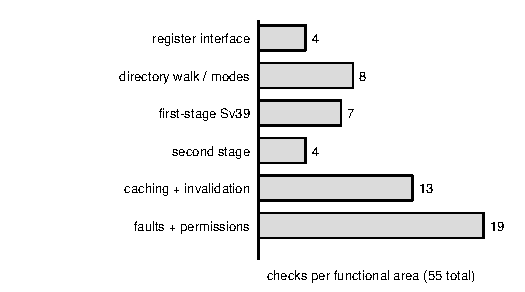
\includegraphics[width=\columnwidth]{figures/figA3_checks.pdf}
\caption{Distribution of the 55 functional checks (a 56th establishes a
precondition).}
\label{fig:checks}
\end{figure}

The suite is 56 checks grouped as in Fig.~\ref{fig:checks}.

\emph{Register interface.} Capability reporting; 4-byte and 8-byte register
access; that a sub-word access does not disturb the following write.

\emph{Directory walk and modes.} \texttt{ddtp} programming including the
two-half commit protocol and the busy handshake; \texttt{Bare} mode passing
transactions through untranslated and performing no directory walk; one-level
directory mode fetching the device context from the expected address
(\texttt{DDT\_BASE} $+$ device identifier $\times$ 32); and that \texttt{ddtp}
can still be reprogrammed after device traffic.

\emph{First-stage translation.} A mapped page translating to the address the
independent walker predicts, with the walk visiting the directory and all three
page-table levels; a second access to the same page served from the IOTLB with
no walk; and 32 randomly chosen mappings accessed at random offsets, each
compared against the walker.

\emph{Second stage.} A device configured with first stage \texttt{Bare} and
second stage Sv39x4, so that the address it emits is a guest physical address;
translation to the expected supervisor address; and that a G-stage entry with
the user bit clear faults, since device accesses are user-mode.

\emph{Caching and invalidation.} That a cached translation survives a
page-table change until invalidated; that \cmd{IOTINVAL.VMA} forces a
re-walk and exposes the new mapping; that an address-scoped invalidation
refreshes the named page and leaves others cached; that an invalidate-all
refreshes every cached page; that \cmd{IOFENCE.C} writes its completion word;
and that no stale translation is observed after that word becomes visible,
including with 24 device accesses in flight throughout.

\emph{Faults and permissions.} An invalid device context, an unmapped address
and \texttt{ddtp}$=$\texttt{Off} each abort the transaction and, importantly,
produce no transaction on the completion port; faulting reads and writes both
receive error responses; faults are recorded in the fault queue; and
page-table entries with the accessed bit clear, the dirty bit clear on a write,
the user bit clear, a reserved bit set, or the valid bit clear each fault.

\begin{table}[!t]
\caption{Test areas, with the number of checks in each}
\label{tab:areas}
\centering\footnotesize
\begin{tabular}{lrl}
\toprule
Area & \# & Representative check \\
\midrule
Register interface    & 4  & 4-byte write takes effect \\
Directory, modes      & 8  & context read from right address \\
First-stage Sv39      & 7  & 32 random maps match walker \\
Second stage Sv39x4   & 4  & GPA maps to expected SPA \\
Caching, invalidation & 13 & no stale entry after fence \\
Faults, permissions   & 19 & dirty bit clear faults a write \\
\midrule
Total                 & 55 & (plus 1 precondition check) \\
\bottomrule
\end{tabular}
\end{table}

Table~\ref{tab:areas} lists the areas. The whole suite builds in 2.4~s and runs
in 5~ms, which matters more than it sounds: a suite that reruns in seconds is a
suite a designer will actually run, and it is what makes the fault-injection
campaign in the next section cheap enough to repeat after every change.

\section{Fault-Injection Evaluation}

\begin{table}[!t]
\caption{Injected faults and whether the suite detects them}
\label{tab:mutants}
\centering\footnotesize
\begin{tabular}{llc}
\toprule
 & Injected defect & Detected \\
\midrule
M1  & first-stage PTE valid bit ignored          & yes \\
M2  & PTE accessed bit ignored                   & yes \\
M3  & PTE dirty bit ignored on stores            & yes \\
M4  & PTE user bit ignored (second stage)        & yes \\
M5  & PTE reserved-bit check removed             & yes \\
M6  & \texttt{ddtp}$=$\texttt{Off} no longer blocks traffic & yes \\
M7  & \texttt{Bare} decoded as a normal mode     & yes$^{\dag}$ \\
M8  & first-stage enable inverted                & yes \\
M9  & IOTLB invalidation does not clear entries  & yes \\
M10 & command-queue head never advances          & yes \\
M11 & invalidate-all clears only the first entry & yes \\
\bottomrule
\end{tabular}
\\[2pt]
\footnotesize $^{\dag}$detected as a hang: the suite fails to complete.
\end{table}

\begin{figure}[!t]
\centering
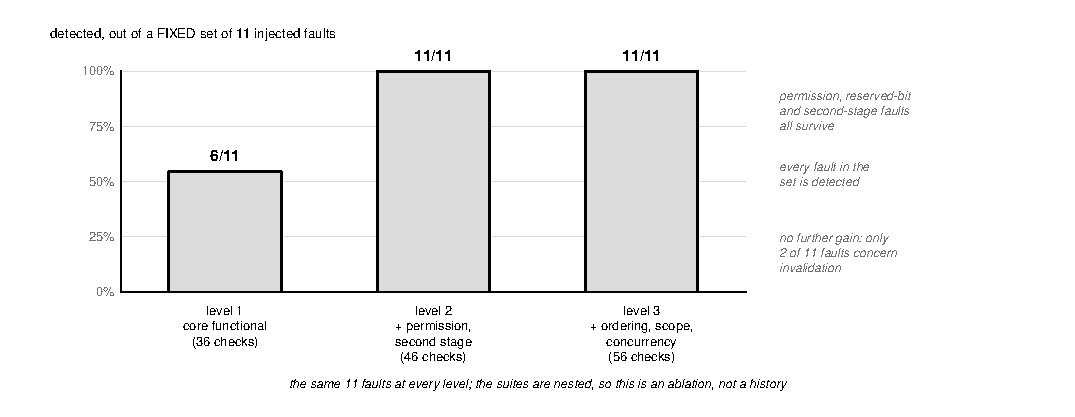
\includegraphics[width=\columnwidth]{figures/figA2_mutation.pdf}
\caption{Detection measured against a fixed set of eleven faults. The suites
are nested, so this is an ablation rather than a history. Level~3 adds no
detection, which reflects the composition of the fault set.}
\label{fig:mut}
\end{figure}

Each fault is one edit to a private copy of the RTL, applied by script; the
suite is rebuilt and rerun, and a fault counts as detected if any check fails.
The faults are chosen to be semantically meaningful rather than syntactic: each
corresponds to an omission a designer could plausibly make.

Table~\ref{tab:mutants} gives the final result, eleven of eleven.

That single number says little on its own, and the way it was reached is easy to
report misleadingly. The suite grew in stages, and so did the fault set; quoting
detection at each stage against the fault set as it then stood would move the
denominator and compare nothing. We therefore fix the fault set at the final
eleven and re-measure every stage of the suite against all of them. The stages
are nested, so this is an ablation rather than a history: level~1 is the core
functional suite, level~2 adds the permission and second-stage tests, level~3
adds the ordering, scope and concurrency tests.

\begin{table}[!t]
\caption{Detection against a fixed set of eleven faults}
\label{tab:ablation}
\centering\footnotesize
\begin{tabular}{@{}clcc@{}}
\toprule
Level & Suite & Checks & Detected \\
\midrule
1 & core functional                        & 36 & 6/11 \\
2 & \quad + permission, second stage       & 46 & 11/11 \\
3 & \quad + ordering, scope, concurrency   & 56 & 11/11 \\
\bottomrule
\end{tabular}
\end{table}

Table~\ref{tab:ablation} reports it. The core suite detects six of the eleven,
and the five it misses are not random: every page-table permission fault
survives, because the core tests always construct entries with the accessed,
dirty and user bits set; the reserved-bit fault survives because they never set
reserved bits; and the second-stage fault survives because they leave the second
stage in \texttt{Bare} mode. Adding tests for those five behaviours detects all
eleven.

The third row is the honest and less comfortable one. The ordering, scope and
concurrency tests---ten further checks, and the subject of a companion
study~\cite{companionB}---raise detection by nothing. We read this as a
statement about the fault set rather than about those tests. Only two of the
eleven faults concern invalidation at all, and both are caught by the core
suite; a set containing faults that break ordering specifically, such as a fence
that reports completion before a preceding invalidation has retired, would
separate level~3 from level~2. A mutation score measures a suite against the
faults one thought to write, and this is what that limitation looks like when it
shows up in one's own data.

This is still the argument for evaluating an environment this way. All 36
level-1 checks passed on the unmodified RTL, and would have passed on an RTL
missing every page-table permission check.

\section{Findings}

\subsection{A faulting device can render the IOMMU unresponsive}
With the fault queue disabled---\texttt{fqcsr.fqen}$=$0---we issue eight
transactions that fault, then a transaction that previously succeeded. The
precondition is checked first: immediately before the experiment, the valid
translation is observed to work. Of the eight faulting accesses, four receive a
response and four receive none. The subsequent valid transaction then fails.

We report this as observed rather than as a specification violation, because the
specification's requirements for fault handling when the queue is disabled are
weaker than for the enabled case, and we did not isolate the internal cause. Its
practical significance does not depend on that adjudication: software that has
not yet enabled the fault queue---during early boot, or after an error---exposes
a path by which a misbehaving or malicious device can stop the IOMMU servicing
transactions at all.

\subsection{Programming sequences are easy to get wrong}
Two behaviours cost us time and would cost an integrator the same. The
\texttt{ddtp} register commits only when both 32-bit halves have been written
and no transaction is in flight, so a single 8-byte write works only because the
bus bridge decomposes it into two 32-bit writes. And the fault queue must be
enabled before faults are provoked, per the finding above. Both are visible in
the RTL; neither is obvious from the register description.

\subsection{A protocol-violating testbench manufactures defects}
\label{sec:false}
During development we recorded three defects in the IP, each reproducible, each
with a plausible mechanism: 4-byte register writes were silently dropped;
\texttt{ddtp} could not be reprogrammed once device traffic had occurred; and a
sub-word access corrupted the following register write.

All three were false. Two independent faults in our own driver produced them.
The driver deasserted \texttt{w\_valid} one cycle late and therefore transferred
two write-data beats for a single-beat burst, leaving a spare beat queued in the
device's bus bridge so that every subsequent write used the \emph{previous}
transaction's data. Separately, it masked sub-word addresses to the 8-byte
boundary, so a 4-byte write to a register at offset \texttt{0x24} was issued at
\texttt{0x20} and wrote the neighbouring register. We found them by monitoring
both sides of the device's internal bridge simultaneously and observing correct
data entering and stale data leaving, with the write-data monitor firing twice
per transaction.

The general point is that the stimulus side of a testbench is unverified code
driving a protocol, and when it violates that protocol the device responds
strangely in ways that are easy to attribute to the device. Every published
``bug'' in a new environment should be treated as a hypothesis about the
testbench until the testbench has been cleared. Protocol checkers are routinely
bound to the device under test; this experience suggests binding them to the
drivers as well.

\section{Discussion}

\subsection{What this would need in a production flow}
The environment here is deliberately small and licence-free, which bounds it.
A production flow would keep three things and replace two. It would keep the
independent walker, because checking a translation against a constant is
worthless once page tables change during a test; it would keep the completion
port as the observation point, because that is where the quantity under test
appears; and it would keep fault injection as the measure of the suite, because
no coverage metric would have told us the permission bits were untested.

It would replace the hand-written drivers with verified bus agents---the
argument of Section~\ref{sec:false} is precisely that hand-written drivers are a
liability---and it would replace the fixed test list with constrained-random
generation over the configuration space: directory depth, page size including
superpages, process contexts, and the interrupt and MSI translation modes this
work does not touch. Functional coverage would then be defined over that space,
with fault injection retained as the check that the coverage model is not
self-satisfied.

\subsection{Generality}
Nothing in the structure is specific to RISC-V. An Arm SMMU presents the same
shape of problem: a stream identifier indexing a table of contexts, two
translation stages, a translation cache, an invalidation command queue with a
completion primitive, and an event queue. The four-component structure, the
independent walker, and the fault-injection evaluation transfer directly; only
the encodings change.

\section{Threats to Validity}
The evaluation measures detection of faults we chose; a different fault set
would give a different score, and eleven of eleven should be read as ``the suite
covers these eleven behaviours,'' not as a general adequacy claim. The
environment exercises one device-directory mode, one process-context
configuration, 4~KiB pages and a 64-bit data bus; superpages, three-level
directories, process contexts, message-signalled interrupt translation,
performance counters and the debug interface are not exercised at all. The IP
does not implement ATS, so no ATS behaviour is tested. All results come from one
simulator; we did not repeat them on a commercial simulator. Finally, the
fault-queue finding is reported as observed behaviour and its specification
status is not settled here.

\section{Conclusion}
An open RISC-V IOMMU implementation of 25{,}778 lines shipped without a
testbench, and without one file needed to lint it. We built an environment that
drives it end to end in 1{,}144 lines using only free tools, and then measured
that environment by injecting defects rather than by counting coverage. The
measurement was worth more than the environment: a suite that passed every check
on the unmodified design would have missed every page-table permission fault,
and only fault injection said so. The same discipline applied to our own
testbench would have saved more time still, since three of the defects we
initially attributed to the device were produced by a driver that did not obey
the bus protocol.

\section*{Artifact Availability}
The environment, the fault-injection harness, the figure scripts and the raw
results are released under a permissive licence. A single command builds the
environment and runs the suite; a second reproduces the fault-injection table.

\begin{thebibliography}{9}
\bibitem{rviommu} Zero-Day Labs, ``RISC-V IOMMU IP,'' commit \texttt{18ad30a}.
[Online]. Available: \url{https://github.com/zero-day-labs/riscv-iommu}
\bibitem{zdl10x} M.~Rodriguez (Zero-Day Labs) and S.~Waheed (10xEngineers),
``Open-source commercial-grade RISC-V IOMMU with verification,'' RISC-V Summit
North America, 2024.
\bibitem{elbrus} A.~A.~Petrykin, I.~A.~Stotland, and A.~N.~Meshkov, ``Standalone
verification of IOMMU with virtualization supporting,'' \emph{Proc. Institute
for System Programming of the RAS}, vol.~31, no.~3, pp.~77--84, 2019.
\bibitem{riscvdv} CHIPS Alliance, ``riscv-dv: random instruction generator for
RISC-V processor verification.'' [Online]. Available:
\url{https://github.com/chipsalliance/riscv-dv}
\bibitem{corevverif} OpenHW Group, ``core-v-verif.'' [Online]. Available:
\url{https://github.com/openhwgroup/core-v-verif}
\bibitem{coatcheck} D.~Lustig, G.~Sethi, M.~Martonosi, and A.~Bhattacharjee,
``COATCheck: Verifying memory ordering at the hardware--OS interface,'' in
\emph{ASPLOS}, 2016.
\bibitem{transform} N.~Hossain, C.~Trippel, and M.~Martonosi,
``TransForm: Formally specifying transistency models and synthesizing enhanced
litmus tests,'' in \emph{ISCA}, 2020.
\bibitem{companionB} M.~Timbadiya, ``Device-side invalidation ordering: testing
IOMMU translation caches at RTL,'' companion article.
\bibitem{rtlcheck} Y.~A.~Manerkar, D.~Lustig, M.~Martonosi, and M.~Pellauer,
``RTLCheck: Verifying the memory consistency of RTL designs,'' in \emph{MICRO},
2017.
\bibitem{verilator} W.~Snyder, ``Verilator.'' [Online]. Available:
\url{https://verilator.org}
\end{thebibliography}

\end{document}
